\chapter{Related Work}
\label{chapter:related}
\epigraph{Hermits United. We meet up every 10 years, swap stories about caves. It’s good fun… for a hermit.}{\textit{The 10th Doctor} - Doctor Who}

\section{Hybrid-Context Sensitivity}

We have discussed directly related work throughout Chapter~\ref{chapter:hybrid}. Here we selectively mention a few techniques that, although not directly related to ours, offer alternative approaches to sweet spots in the precision/performance tradeoff.

Special-purpose combinations of context sensitivity have been used in the past, but have required manual identification of classes to be treated separately (e.g., Java collection classes, or library factory methods). An excellent representative is the TAJ work for taint analysis of Java web applications \cite{pldi:2009:Tripp}. In contrast, we have sought to map the space and identify interesting hybrids for general application of context sensitivity, over the entire program.

The analyses we examined are context-sensitive but flow-insensitive. We can achieve several of the benefits of flow sensitivity by applying the analysis on the static single assignment (SSA) intermediate form of the program. This is easy to do with a mere flag setting on the \doop{} framework. However, the impact of the SSA transformation on the input is minimal. The default intermediate language used as input in \doop{} (the Jimple representation of the Soot framework \cite{cascon:1999:Vall,cc:2000:Vall}) is already close to SSA form, although it does not guarantee that every variable is strictly single-assignment without requesting it explicitly. Published work by Lhot\'{a}k and Chung \cite{popl:2011:Lhotak} has shown that much of the benefit of flow sensitivity derives from the ability to do strong updates of the points-to information. Lhot\'{a}k and Chung then exploited this insight to derive analyses with similar benefit to a full flow-sensitive analysis at lower cost.

A demand-driven evaluation strategy reduces the cost of an analysis by computing only those results that are necessary for a client program analysis~\cite{oopsla:2005:Sridharan,pldi:2006:Sridharan,popl:2008:Zheng,pldi:2001:Heintze}. This is a useful approach for client analyses that focus on specific locations in a program, but if the client needs results from the entire program, then demand-driven analysis is typically slower than an exhaustive analysis.

Reps~\cite{cc:1994:Reps} showed how to use the standard magic-sets optimization to automatically derive a demand-driven analysis from an exhaustive analysis (like ours). This optimization combines the benefits of top-down and bottom-up evaluation of logic programs by adding side-conditions to rules that limit the computation to just the required data.

An interesting recent approach to demand-driven analyses was introduced by Liang and Naik \cite{pldi:2011:Liang}. Their ``pruning'' approach consists of first computing a coarse over-approximation of the points-to information, while keeping the provenance of this derivation, i.e., recording which input facts have affected each part of the output. The input program is then pruned so that parts that did not affect the interesting points of the output are eliminated. Then a precise analysis is run, in order to establish the desired property.



\section{Introspective Analysis}
\label{sec:related:introspective}

The effort to tune the context sensitivity of an analysis is pervasive in the literature. Nevertheless, most approaches fundamentally differ from ours of Chapter~\ref{chapter:introspective}, either by trying to vary context sensitivity based on syntactic properties or by trying to focus on only a part of the program that matters for answering a given query. In contrast, we attack the context-sensitive scalability problem  head-on, in the all-points points-to analysis setting, with context used all over the program and library.

Typical scalable points-to analysis frameworks such as \textsc{Wala}~\cite{www:wala} and \doop{}~\cite{oopsla:2009:Bravenboer} employ a multitude of low-level heuristics for tuning the precision and scalability of an analysis. These include using extra context for collection classes, using a heap context for arrays in an analysis without a context-sensitive heap, allocating strings or exceptions context-insensitively, treating library factory methods with deeper context, etc. Such heuristics are typically user-selected and prominent in the documentation of the respective frameworks, and have also appeared in the literature (e.g., \cite{pldi:2009:Tripp,cc:2013:Kastrinis}). However, all such approaches are mere hard-wired heuristics and do not address the major scalability problem that our approach aims to solve. The scalability issues identified in earlier literature and discussed throughout this paper are present after all such heuristics have been employed.

A more general approach is the hybrid-context sensitivity of Chapter~\ref{chapter:hybrid}. Such a hybrid analysis attempts to emulate call-site sensitivity for static method calls and object sensitivity for dynamic calls. The approach becomes interesting when context is deep (e.g., how are context elements merged when a dynamic call is made inside a static call?). Nevertheless, the hybrid-context sensitivity approach does not change the essence of the problem we are trying to solve. For hard-to-analyze applications, hybrid context-sensitive algorithms are equally unscalable as their component algorithms. For the purposes of our experimental study, which only tests the scalability of heavyweight benchmarks, hybrid-context sensitivity is virtually indistinguishable from object sensitivity.

In recent years there have been many more instantiations of introspective analysis, with very different metrics of cost and benefit. These modern instantiations outperform our original Heuristic-A and Heuristic-B but keep the same flavor: \textsc{Zipper}~\cite{oopsla:2018:Li} aims to achieve mostly-guaranteed precision with heuristically better scalability, whereas \textsc{Scaler}~\cite{esec-fse:2018:Li} achieves guaranteed scalability and typically significantly better precision than a context-insensitive analysis.

More interesting applications of selective context sensitivity have been explored in the context of \emph{demand-driven} pointer analysis. A demand-driven evaluation strategy reduces the cost of an analysis by computing only those results that are necessary for a client program analysis~\cite{oopsla:2005:Sridharan,pldi:2006:Sridharan,popl:2008:Zheng,pldi:2001:Heintze}. This is a useful approach for client analyses that focus on specific locations in a program, but if the client needs results from the entire program, then demand-driven analysis is typically slower than an exhaustive analysis.

In the demand-driven space, refinement-based analyses have been used primarily in the work of Sridharan and Bod\'{\i}k~\cite{pldi:2006:Sridharan} and of Liang and Naik~\cite{pldi:2011:Liang}. Sridharan and Bod\'{\i}k introduce refinement-based analysis as a way to adaptively increase the precision characteristics of an existing analysis algorithm when a client analysis is not satisfied with the result. The approach allows turning on field sensitivity, as well as higher call-site sensitivity for an analysis algorithm. Yet, unlike ours, it is not a general approach that can apply to any kind of context and a large number of different algorithms. Liang and Naik's ``pruning'' approach consists of first computing a coarse over-approximation of the points-to information, while keeping the provenance of this derivation, i.e., recording which input facts have affected each part of the output. The input program is then pruned so that parts that did not affect the interesting points of the output are eliminated. Then a highly context-sensitive precise analysis is run, in order to establish the desired property. This approach is similar to introspective context sensitivity in that the analysis is run twice and a separate query over the first-run result determines the second run's characteristics. Nevertheless, our approach requires no provenance computation (which is unlikely to scale for an all-points analysis) and works even when we want answers for the entire program---i.e., when pruning is not possible.

Both of the above demand-driven approaches can be viewed as complements of our introspective context sensitivity. In the demand-driven world, it is possible to estimate the \emph{benefit} that a more precise analysis may yield: either the client is happy with the current level of precision (which implies there is no further benefit to be obtained) or it is not, in which case more precision should be added. In our all-points pointer analysis problem we have no such information. This motivates our \emph{cost}-based heuristics, which attempt to estimate ``what can go wrong'' when more precision gets added, as opposed to ``what can be gained'', as in demand-driven techniques.



\section{Must-Alias Analysis}

\subsection*{Logical Model}

There are several approaches in the literature that present must-analyses in the pointer analysis setting or employ them in a may-analysis. Our approach is a must-alias analysis applied to Java bytecode, but conceptually it is distinguished by its minimizing the distance between the implementation and the declarative specification.

Ma et al.~\cite{isola:2008:Ma} present an algorithm for null-pointer dereference detection using a context-insensitive may-alias and a must-alias analysis; the latter is used to increase the precision of the former, by enabling strong updates when possible.

Nikoli\'{c} and Spoto~\cite{ictac:2012:Nikolic} present a must-alias analysis that tracks aliases between program expressions and local variables (or stack locations, since they analyze Java bytecode, which is a stack-based representation). The analysis is related to ours both because of its application to Java bytecode and because it is constraint-based: the analysis is a generator of constraints, which are subsequently solved to produce the analysis results. Abstractly, this is a relative of our Datalog-based approach, but it is unclear how the two may compare in terms of engineering tradeoffs.

Hind et al. \cite{article:1999:Hind} present a collection of pointer analysis algorithms. Among them, the most relevant to this work is a flow-sensitive interprocedural pointer alias analysis. The authors optimistically produce \emph{must} information for pointers to single non-summary objects.

Emami et al.~\cite{pldi:1994:Emami} present an approach that simultaneously calculates both must- and may-point-to information for a C analysis. Their empirical results ``show the existence of a substantial number of definite points-to relationships, which forms very valuable information''---much in line with our own experience.

The analysis of \cite{ecoop:2012:De} is essentially a flow-sensitive may-point-to analysis that performs strong updates, as it maps \emph{access paths} to \emph{heap objects} (abstracted by their allocation sites). The approach uses a flow-insensitive may-point-to analysis to bootstrap the main analysis. However, it provides no \emph{definite} knowledge of any sort, since the aim is to increase the precision of the may-analysis. For instance, even if an access path points to a single heap object, according to the De and D'Souza analysis, there is no \emph{must} point-to information derived, since this object could be a summary object (i.e., one that abstracts many objects allocated at the same allocation site). To reason about such cases, other approaches, such as the more expensive shape analysis algorithms \cite{article:2002:Sagiv}, additionally maintain summary information per heap object. In this way, they allow must point-to edges to exist only if the target is definitely not a summary node.

Must- information is often computed in conjunction with a client analysis. One of the best examples is the typestate verification of Fink et al.~\cite{issta:2006:Fink}, which demonstrates the value of a must-analysis and the techniques that enable it.

An approach for integrating \emph{must} point-to reasoning in an analysis is to propagate such information only at instructions where we know that the given heap allocation target still refers to the last object allocated at that site \cite{popl:1995:Altucher}. Thus, an execution path that may create another object at the same site (such as when reaching the end of the loop) would invalidate any previous must-point-to facts (i.e., it will stop them from propagating any further).

Generally, must-analyses can vary greatly in sophistication and can be employed in an array of different combinations with may-analyses. The analysis of Balakrishnan and Reps~\cite{sas:2006:Balakrishnan}, which introduces the \emph{recency abstraction}, distinguishes between the most recently allocated object at an allocation site (a concrete object, allowing strong updates) and earlier-allocated objects (represented as a summary node). The analysis additionally keeps information on the size of the set of objects represented by a summary node. At the extreme, one can find full-blown shape analysis approaches, such as that of Sagiv et al.~\cite{article:2002:Sagiv}, which explicitly maintains must- and may- information simultaneously, by means of three-valued truth values, in full detail up to predicate abstraction: a relationship can definitely hold (``must''), definitely not hold (``must not'', i.e., negation of ``may''), or possibly hold (``may''). Summary and concrete nodes are again used to represent knowledge, albeit in full detail, as captured by arbitrary predicates whose value is maintained across program statements, at the cost of a super-exponential, worst-case complexity.

Jagannathan et al.~\cite{popl:1998:Jagannathan} present an algorithm for must-alias analysis of functional languages. The algorithm adapts must-alias insights to the setting of captured variables in closures. For instance, must-alias information for non-summary objects permits strong updates, which the authors find to improve analysis precision. We employ must-alias analysis results quite similarly in applications of our model analysis.


\subsection*{Data Structures}

Our optimized data structure is (partly) based on the observation that must-alias sets are equivalence classes. This is not the first time that a data structure that efficiently implements equivalence classes has been used to speed up pointer analysis. Most notably, a Steensgaard-style (or \emph{unification-based}) \cite{popl:1996:Steensgaard} analysis computes may-point-to sets that are equivalence classes. This means that points-to sets are disjoint---if two points-to sets are found to possibly overlap, they get unified. This loses precision (relative to a standard subset-based points-to analysis) but enables the algorithm to use union-find trees for a very efficient representation.

Another optimized data structure often used in pointer analysis is the \emph{constraint graph}: a graph with nodes denoting pointer variables and an edge between nodes \code{p} and \code{q} denoting flow (e.g., a direct assignment) from variable \code{p} to variable \code{q}. Online cycle elimination by F\"{a}ndrich et al. \cite{pldi:1998:Fahndrich} detects cycles in the constraint graph and collapses all nodes in a cycle into a representative node, since such nodes will have identical points-to information. The technique of Nasre \cite{ismm:2012:Nasre} extends such constraint graph reasoning based on the observation that if two nodes have the same dominator in the constraint graph, then they are clones: the values flowing to them are (only) those of the dominator node. Several other constraint graph optimizations are applied off-line (i.e., before the points-to analysis runs). Prime examples of such techniques are Rountev and Chandra's \cite{pldi:2000:Rountev} and Hardekopf and Lin's \cite{sas:2007:Hardekopf}. (Hardekopf and Lin have also applied similar ideas in a hybrid online/offline setting \cite{pldi:2007:Hardekopf}.) Both of these techniques perform an off-line detection of equivalent points-to sets and use this knowledge to eliminate redundant work in subsequent points-to computations. Our data structure can be seen as somewhat analogous to constraint-graph techniques, in the sense that we do not compute the flow of objects or the fully expanded set of all possible alias pairs. Instead, we compute the ``wiring'' (i.e., the alias relationships, locally, that the program induces) and keep the alias information in condensed form, until it needs to be queried by a client analysis.

Another conceptual relative of our data structure is the model presented by Madhavan et al. \cite{article:2015:Madhavan} for modular may-analyses. That model is similar in that it invents abstract nodes for heap objects that resemble ours (without the equivalence-class nature). The Madhavan et al. approach aims to achieve modular reasoning, i.e., to model the heap effects of a method without knowing its calling environment. To do so, the approach creates abstract nodes that represent concepts such as ``whichever object variable \code{x} may point to''. Our data structure has nodes with a similar meaning, however we also take advantage of the ``must'' nature of the analysis to merge nodes, every time the same access path can reach both.



\section{Defensive Analysis}
\label{sec:related:defensive}

There is certainly past work that attempt to ensure a sound whole-program analysis, but none matches the generality and applicability of our approach. We selectively discuss representative approaches.

The standard past approach to soundness for a careful static analysis has been to ``bail out'': the analysis detects whether there are program features that it does not handle soundly, and issues warnings, or refuses to produce answers. This is a common pattern in abstract-interpretation~\cite{popl:1977:Cousot} analyses, such as Astr\'{e}e~\cite{sas:2007:Delmas}, which have traditionally emphasized sound handling of conventional language features. However, this is far from a solution to the problem of being sound for opaque code: refusing to handle the vast majority of realistic programs can be argued to be sound, but is not usefully so. In contrast, our work handles \emph{all} realistic programs, but returns partial (but sound) results, i.e., produces non-empty points-to sets for a subset of the variables. It is an experimental question to determine whether this subset is usefully large, as we do in our evaluation.

Hirzel et al. \cite{ecoop:2004:Hirzel,article:2007:Hirzel} use an online pointer analysis to deal with reflection and dynamic loading by monitoring their run-time occurrence, recording their results, and running the analysis again, incrementally. However, this is hardly a \emph{static} analysis and its cost is prohibitive for precise (context-sensitive) analyses, if applied to all reflection actions.

Lattner et al. \cite{pldi:2007:Lattner} offer an algorithm that can apply to incomplete programs, but it assumes that the linker can know all callers (i.e., there is no reflection---the analysis is for C/C++) and the approach is closely tied to a specific flow-insensitive, unification-based analysis logic~\cite{popl:1996:Steensgaard}, necessary for simultaneously computing inter-related points-to, may-alias, and may-escape information.

Sreedhar et al. \cite{pldi:2000:Sreedhar} present the only past approach to explicitly target dynamic class loading, although only for a specific client analysis (call specialization). Still, that work ends up making many statically unsound assumptions (requiring, at the very least, programmer intervention), illustrating well the difficulty of the problem, if not addressed defensively. The approach assumes that only the public API of a ``closed world'' is callable, thus ignoring many uses of reflection. (With reflection, any method is callable from unknown code, and any field is accessible.) It ``[does] not address the Java features of reloading and the Java Native Interface''. It ``optimistically assumes'' that ``[the extant state of statically known objects] remains unchanged when they become reachable from static reference variables''. It is not clear whether the technique is conservative relative to adversarial native code (in system libraries, since the JNI is ignored). Finally, the approach assumes the existence of a sound may-point-to analysis, even though none exists in practice!

Traditional conservative call-graph construction (\emph{Class Hierarchy Analysis (CHA)} \cite{ecoop:1995:Dean} or \emph{Rapid Type Analysis (RTA)} \cite{oopsla:1996:Bacon}) is unsound. Such algorithms explore the entire class hierarchy for matching (overriding) methods and consider all of them to be potential virtual call targets. However, even this is not sufficient for a sound static analysis of opaque code: classes can be generated and loaded dynamically during program execution. CHA cannot find target methods that do not even exist statically, yet modeling them is precisely what is needed for soundness in real-world conditions. For instance, Java applications, especially in the enterprise (server-side) space, employ dynamic loading heavily, and patterns such as \emph{dynamic proxies} have been standardized and used widely since the early Java days.

Furthermore, such heuristic ``best-effort'' over-approximation is detrimental to analysis precision and performance. CHA is an example of a loose over-approximation in an effort to capture most dynamic behaviors.
(Similar loose over-approximations have been proposed, for instance, for reflection analysis~\cite{aplas:2015:Smaragdakis}.) Loose over-approximations compute many more possible targets than those that realistically arise. This yields vast points-to sets that render the analysis heavyweight and useless due to imprecision. (Avoiding such costs is exactly why past analyses have often opted for glaringly unsound handling of opaque code features.) Our lazy representation of ``don't know''/''cannot bound'' values as empty sets addresses the problem, by keeping all points-to sets compact.

The conventional handling of reflection in may-point-to analysis algorithms for Java~\cite{www:wala-reflection,ecoop:2014:Li,aplas:2005:Livshits,thesis:Livshits,aplas:2015:Smaragdakis,sas:2015:Li} is unsound, instead relying on a ``best-effort'' approach.  Such past analyses attempt to statically model the result of reflection operations, e.g., by computing a superset of the strings that can be used as arguments to a \code{Class.forName} operation (which accepts a name string and returns a reflection object representing the class with that name). The analyses are unsound when faced with a completely unknown string: instead of assuming that \emph{any} class object can be returned, the analysis assumes that \emph{none} can. The reason is that over-approximation (assuming any object is returned) would be detrimental to the analysis performance and precision. Even with an unsound approach, current algorithms are heavily burdened by the use of reflection analysis. For instance, the documentation of the \textsc{Wala} library directly blames reflection analysis for scalability shortcomings \cite{www:wala-reflection},\footnote{The \textsc{Wala} documentation is explicit: ``\emph{Reflection usage and the size of modern libraries/frameworks make it very difficult to scale flow-insensitive points-to analysis to modern Java programs. For example, with default settings, \textsc{Wala}'s pointer analyses cannot handle any program linked against the Java 6 standard libraries, due to extensive reflection in the libraries.}''~\cite{www:wala-reflection}} and enabling reflection on the \doop{} framework slows it down by an order of magnitude on standard benchmarks~\cite{aplas:2015:Smaragdakis}. Furthermore, none of these approaches attempt to model dynamic loading---a ubiquitous feature in Java enterprise applications.



\section{General Directions in Program Analysis}

Finally, in this section, we extend our focus on the broader area of (static) program analysis and automatic program understanding. We touch upon various methodologies that have been introduced in past literature aiming to tackle more or less similar issues to the ones previously discussed.


\subsection{Control-Flow Analysis (\texorpdfstring{$k$}{k}-CFA)}

The term \emph{control-flow analysis} (CFA) commonly describes an algorithm incorporating both data-flow and control-flow reasoning, and more specifically, in which data-flow depends on control-flow, and at the same time, control-flow depends on data-flow. In the setup of our work, points-to reasoning plays the part of data-flow and call-graph reasoning plays the part of control-flow. But, control-flow analysis is not strictly confined to the setting of pointer analysis in object-oriented languages. It can also apply to functional languages in a similar problem known as \emph{flow analysis}---in which variables may a value flow to? Both settings introduce a degree of complexity due to higher-order features; functional languages have first-class functions and object-oriented languages have dynamic dispatch.

The origin of $k$-CFA is found in Shivers's dissertation \cite{thesis:Shivers}, and was developed to solve the higher-order control-flow problem in $\lambda$-calculus-based languages. Consequently, it applies both in functional languages that are explicitly vulnerable to the issue because closures are passed around as first-class values, and in object-oriented languages where the issue is more implicit in method invocations being resolved dynamically.

$k$-CFA is a well-known family of control-flow analysis algorithms, widely recognized in both communities that popularized the idea of context-sensitive flow analysis. Although, in the setting of object-oriented languages, $k$-CFA is often made synonymous to ``context-sensitive-to-depth-$k$'' it is in fact an algorithm that incorporates context sensitivity along with several other design decisions. Nevertheless, informally, $k$-CFA commonly refers to a $k$-call-site-sensitive analysis with a $k$-context-sensitive heap.


\subsection{CFL Reachability Formulation}

In previous chapters we either formulated pointer analysis algorithms directly as Datalog rules, or in the case of defensive analysis (Chapter~\ref{chapter:defensive}) as inference rules that can be translated to Datalog rules in a straightforward fashion. This minimalistic approach allows one to better reason about the way that language features interact with each other when designing an analysis algorithm, without the burden of taking implementation details into account. Additionally, such formulation can easily offer time and space complexity bounds for the analysis under development as well as termination guarantees for the resulting algorithm. Furthermore, as an added bonus, the Datalog specification is quite close to the actual implementation of the algorithm in a Datalog engine.

Several past pointer analysis algorithms (as well as other related analyses) have been formulated as a \emph{context-free language (CFL) reachability} problem \cite{ilps:1997:Reps} that can later be translated into Datalog rules. The core idea is that one encodes an input program as a labeled graph, and a specific analysis as a context-free grammar, $G$. The relation being computed by the analysis (e.g., aliasing information) holds for two nodes of the graph iff there exists a path from one node to the other, such that concatenating the labels on the edges along that path gives a string that belongs to the language $L(G)$ defined by the aforementioned grammar.

In more detail, nodes in the input graph represent program elements such as variables, methods, types, statements, and so on. Edges represent relations between such nodes. For instance, an edge $e(s, t)$ may represent a local assignment statement for the variables encoded in graph nodes $s$ and $t$. Other common edge encodings include field accesses (load/stores), method invocations, pointer dereferences, etc. The exact choice of domains depends on the actual analysis that is being designed each time. In order to encode many different input relations simultaneously on the graph, different kinds of edges can be employed. For a given analysis, a context-free grammar $G$ encodes the desired computed attributes as non-terminal symbols, and supplies production rules that express how they relate to the simpler relations represented by graph edges---and terminals in the grammar. The CFL reachability solution in then commonly computed using a dynamic programming algorithm.

The first application of CFL reachability in program analysis intended to solve various interprocedural dataflow-analysis problems \cite{popl:1995:Reps,pppj:2014:Milanova}, but since then is has been used in a wide range of problems, such as:
\begin{inparaenum}[(1)]
\item program slicing \cite{fse:1994:Reps} (more on that later),
\item shape analysis \cite{pepm:1995:Reps},
\item the computation of points-to relations \cite{article:1998:Reps,cgo:2012:Lei,pldi:2006:Sridharan,oopsla:2005:Sridharan,ecoop:2009:Xu,cc:2013:Lu},
\item the demand-driven computation of may-alias pairs in a C-like language \cite{popl:2008:Zheng},
\item Andersen-style pointer analysis for Java \cite{oopsla:2005:Sridharan}.
\end{inparaenum}

As previously mentioned, any CFL reachability problem can be converted to a Datalog program \cite{article:1998:Reps}, but not the other way around. In that sense, CFL reachability implicitly corresponds to a restricted subset of Datalog programs, often called \emph{chain programs}. As a consequence, the core advantage of CFL reachability is that it describes Datalog programs that allow for more efficient implementations. In this setting, Datalog relations represent labeled edges in the graph. For instance, the fact \rel{P}{X, Y} encodes that node \args{X} and node \args{Y} are connected via an edge labeled \relname{P}. A chain program consists of rules of the following form:

\begin{displayquote}
\begin{datalog}
\rel{P}{X, Y} \dlIf{} \rel{Q\textsubscript{0}}{X, Z\textsubscript{1}}, \rel{Q\textsubscript{1}}{Z\textsubscript{1}, Z\textsubscript{2}}, ..., \rel{Q\textsubscript{k}}{Z\textsubscript{k}, Y}.
\end{datalog}
\end{displayquote}

The corresponding grammar $G$ provides production rules as the following:

\begin{displayquote}
\begin{datalog}
\relname{$P$} \dlIfInv{} \relname{$Q_0$} \relname{$Q_1$} ... \relname{$Q_k$}
\end{datalog}
\end{displayquote}

A more concrete example, related to pointer analysis, is given in the following production rule that describes how information (i.e., abstract objects) flow from the point of allocation, through various assignments, to reach a program expression (e.g., variable).

\begin{displayquote}
\begin{datalog}
\relname{$FlowsTo$} \dlIfInv{} \relname{$Alloc$} ( \relname{$Assign$} ) *
\end{datalog}
\end{displayquote}

The graph in Figure~\ref{fig:related:cfl} encodes a small code snippet identified by the previous production rule.

\begin{figure}[ht]
\centering
% left bottom right top
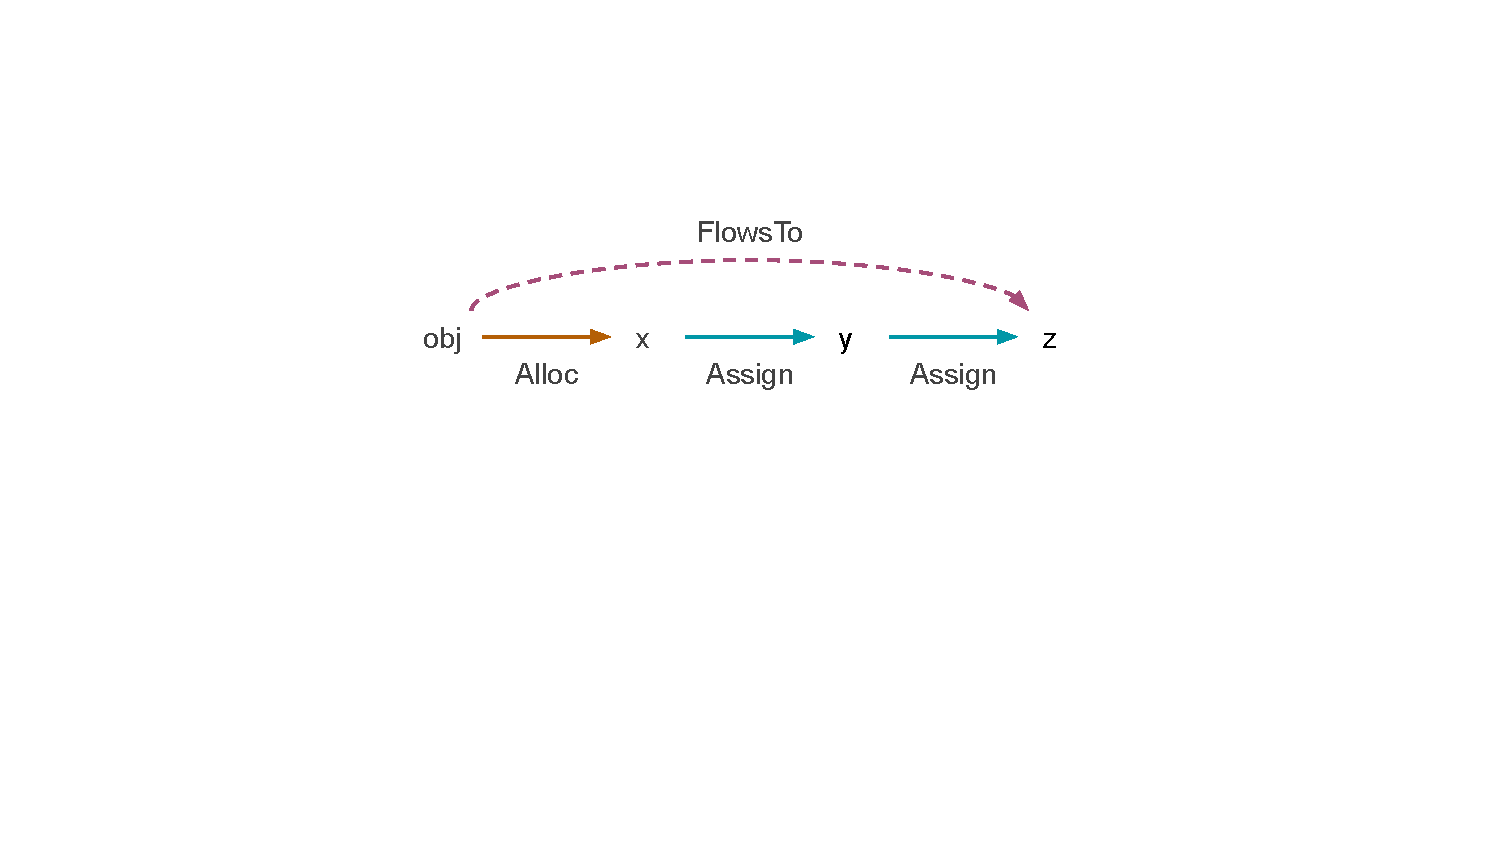
\includegraphics[trim={40mm 75mm 40mm 35mm},clip,width=1\linewidth]{assets/related/CFL.pdf}
\caption[Example of a CFL-Reachability Graph]{Example of a CFL Reachability Graph.}
\label{fig:related:cfl}
\end{figure}

Initially, an abstract object \args{obj} is allocated to variable \code{x}. Then, \code{x} is assigned to \code{y} and \code{y} is assigned to \code{z}. Subsequently, an indirect flow is inferred from object \args{obj} to variable \code{z}.


\paragraph{Dyck-CFL Reachability.}
A more restrictive variant is that of \emph{Dyck-CFL reachability}. Restrictions on the underlying context-free grammar result in a \emph{Dyck} language, i.e., one that generates balanced-parentheses expressions. This restrictive approach still suffices for certain simple pointer analysis algorithms and at the same time it enables very aggressive performance optimizations \cite{pldi:2013:Zhang,esop:2009:Yuan}.

Figure~\ref{fig:related:dyck-cfl} gives a simple example of a graph corresponding to a Dyck grammar. An opening parenthesis encodes a field store, and a closing one encodes a field load. In both cases, the field being accessed is used as subscript to differentiate different fields.

\begin{figure}[ht]
\centering
% left bottom right top
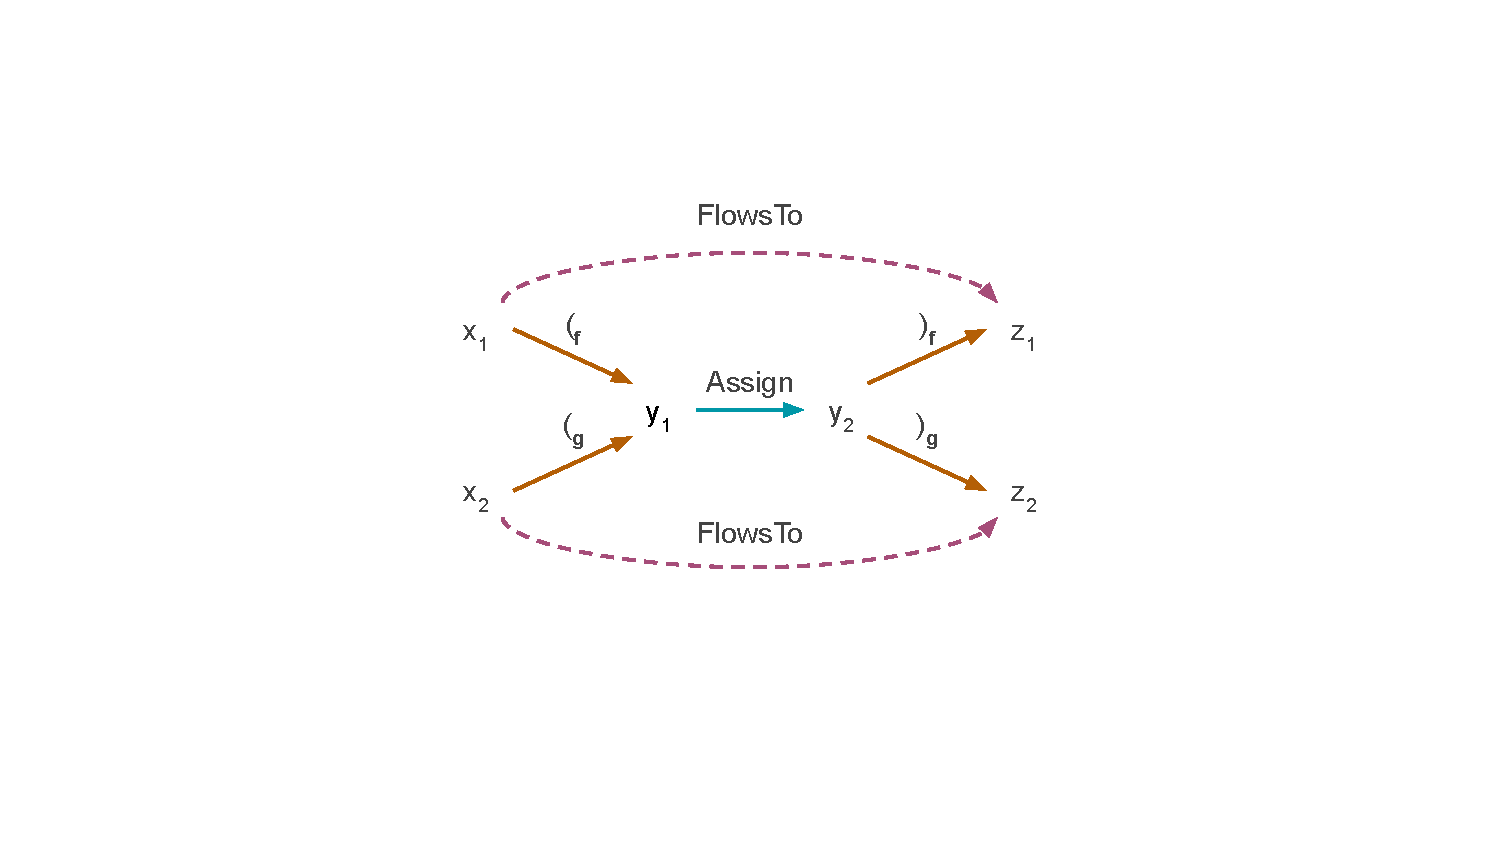
\includegraphics[trim={40mm 40mm 40mm 30mm},clip,width=1\linewidth]{assets/related/DyckCFL.pdf}
\caption[Example of a Dyck-CFL-Reachability Graph]{Example of a Dyck-CFL Reachability Graph.}
\label{fig:related:dyck-cfl}
\end{figure}

The field differentiation of parentheses avoids erroneous inferences, such as the value of \codeRAW{x\textsubscript{2}} flowing into \codeRAW{z\textsubscript{1}}. The corresponding Dyck grammar includes productions rules as the following:

\begin{displayquote}
\begin{datalog}
\relname{$FlowsTo$} \dlIfInv{} \relname{$Assign$} | ($_f$ \relname{$FlowsTo$} )$_f$ | ($_g$ \relname{$FlowsTo$} )$_g$ | ...
\end{datalog}
\end{displayquote}


\subsection{Probabilistic Pointer Analysis}

As previously mentioned, pointer analysis has evolved into a critical tool for compiler analysis and optimizations. Many sophisticated optimizations enforced by a compiler need some kind of proof that certain properties hold in order to guarantee that the compilation process does not introduce errors into the program.

To that end, one approach is to either use some variation of a \emph{must} analysis (as in Chapters~\ref{chapter:must-logic} and \ref{chapter:must-data}), or a \emph{sound-may} analysis (as in Chapter~\ref{chapter:defensive}) and look at the complement of the result (i.e, if a sound-may analysis claims a set of behaviors may apply to a certain point in the program, then the compiler is certain that no other behavior may arise).

On the other hand, compilers in recent years have another potential direction to follow; that of \emph{speculative optimizations}. A speculative optimization typically involves a code transformation that allows ambiguous memory references to be scheduled in a potentially unsafe order, and requires a recovery mechanism to ensure program correctness. Nowadays, speculative optimizations are widely used in the compilation pipeline, which allows compilers to employ the results of a \emph{may} analysis as well. The very nature of those optimizations means that they are accompanied with safeguards for when applying them was not the correct choice. Thus, a compiler can aggressively exploit information from an analysis that is not always guaranteed to hold.

More aggressive, hardware-supported techniques, such as thread-level speculations \cite{asplos:1998:Hammond,article:1999:Krishnan,hpca:2001:Roth} and transactional programming \cite{article:2004:Hammond,asplos:1998:Hammond} apply speculative parallelization of sequential programs by utilizing specialized hardware. The downside is that many of these optimizations rely on extensive data dependence profiling in order to decide when to speculate. Such information is expensive to acquire or potentially unavailable.

This has led to the family of \emph{probabilistic pointer analysis} algorithms \cite{asplos:2006:Silva,aplas:2007:DiPierro,article:2004:PengSheng} that aim to compute pointer information accompanied with some amount of likelihood. These algorithms provide an alternative approach to profiling. Since they are an instance of a static analysis, they can be employed at compile-time to alleviate the aforementioned lack of profile information.

A probabilistic pointer analysis algorithms statically predict the probability of each points-to relation at each program point. Such probabilities are especially useful to a compiler when applying some kind of speculative optimization. Beside more traditional techniques (for instance, static or dynamic profiling), various statistics concepts and stochastic models (e.g., sparse transformation matrices, Discrete-Time Markov chains, etc.) from other fields have been imported into the domain of static analysis for this purpose.


\subsection{Recency Abstraction}

Any static analysis algorithm will construct an abstraction model of the program's memory, with a single \emph{abstract} heap object potentially encoding multiple \emph{concrete} (runtime) objects. The most common approach is (as already discussed in previous chapters) to use each allocation instruction to encode a single abstract object in memory.

A different approach is offered by \citeauthor{sas:2006:Balakrishnan} \cite{sas:2006:Balakrishnan} in their \emph{recency-abstraction} technique. In that approach, each allocation site encodes \emph{two} abstract memory objects:
\begin{inparaenum}[(1)]
\item one that represents the \emph{most-recently-allocated} object (for that allocation site), and
\item one that summarizes all other, previously allocated objects.
\end{inparaenum}
An analysis can exploit this most-recently-allocated object, since it represents a single concrete runtime object, and apply ``strong updates'' reasoning. This proves essential in improving precision and scalability on a flow-sensitive analysis.


\subsection{Separation Logic (\& Hoare Logic)}

Pointer analysis ultimately constructs a model of the heap, by computing all the heap objects that each program expression may point to during execution. But, this is by no means the only approach that analyzes the heap. Other approaches, that stem from the field of \emph{separation logic} \cite{lics:2002:Reynolds,csl:2001:OHearn,popl:2001:Ishtiaq,col:2000:Reynolds,article:2011:Calcagno,article:2012:OHearn}, have been used to reason about the heap and produce proofs regarding pointer safety. Separation logic, in turn, extends the theory of \emph{Hoare logic} \cite{article:1981:Krzysztof}.

Hoare logic provides a formal system to reason about program correctness, by encoding a language's semantics (and therefore the program's as well) in \emph{Hoare triples}. A Hoare triple has the form $\{P\} \; C \;  \{Q\}$, and encodes that whenever an assertion $P$ holds, before executing command $C$, then assertion $Q$ is quaranteed to hold afterwards---if $C$ terminates. The $P$ and $Q$ assertions express conditions on local variables---written in standard mathematical notation alongside some form of calculus (e.g., \emph{first-order logic}).

Hoare logic provides two variants of operation:
\begin{inparaenum}[(1)]
\item a forward approach in which one starts from a precondition and generates formulas in order to prove a postcondition,
\item and a backwards approach in which the opposite direction is followed (i.e., start from a postcondition and prove a precondition).
\end{inparaenum}
In the general case, regardless of which variant is employed, the process cannot result in a fully automated reasoning and building a general proof may require human guidance to some extent.

Separation logic builds upon Hoare logic by introducing additional operators in the syntax of assertions that focus on local reasoning. For instance, the \emph{separating conjunction} operator, $P \; * \; Q$, asserts that conditions $P$ and $Q$ hold for separate parts of memory, and thus can be used on program proofs to enable modular reasoning. Another interesting operator is that of \emph{separating implication}, $P \mathrel{-\mkern-6mu*} \; Q$, which asserts that if the current heap is extended with a part where $P$ holds, then $Q$ holds in the extended heap. It is noteworthy that, despite all of its extensions, separation logic is not more ``powerful'' than Hoare logic---all that is provable in separation logic is also provable in Hoare logic. The extensions serve to simplify the specifications and proofs.

For example, the condition ($x \mapsto y \; * \; y \mapsto x$) asserts that $x$ points to $y$ and separately $y$ points to $x$. This formula describes \emph{precisely} two allocated memory parts---denoted by $x$ and $y$---i.e., it is guaranteed that the pointers do not alias.

A simple example of a separation logic rule, given some resource $r$, is the following: 
\[
\{ \; isOpen(r) \; \} \; \codeRAW{closeRes(r)} \; \{ \; isClosed(r) \; \}
\]
This rule describes a \emph{specification} for a method \code{closeRes} that given a resource handler $r$, closes that resource. Now, given a precondition $\{isOpen(r_1) \; * \; isOpen(r_2)\}$ one can infer the following formula:
\[
\{ \; isOpen(r_1) \; * \; isOpen(r_2) \; \} \; \codeRAW{closeRes(r\textsubscript{1})} \; \{ \; isClosed(r_1) \; * \; isOpen(r_2) \; \}
\]
This highlights how separating conjunction allows one to reason about mutations in memory, mimicking the actual updates happening in RAM during execution. Such reasoning leads to logical proofs about imperative programs that match computational intuition.

The previous formula expansion is based on a general pattern in separation logic; a \emph{frame rule} that allows one to go from smaller to bigger specifications. It is named after the classic frame problem found in artificial intelligence. Here $frame$ describes a part of the program state that remains unchanged after the semantics of command $C$ have been applied.
\[
\frac
{\{P\} \; C \;  \{Q\}}
{\{P \; * \; frame \} \; C \;  \{Q \; * \; frame \}}
\]
The frame rule is key to local reasoning in separation logic; reasoning and specifications should concentrate on the resources that are affected by a given command, without mentioning what remains unchanged.

\paragraph{Bi-abduction.}
In classical logic, entailment statements, such as $A \; \vdash \; G$, denote that $A$ implies $G$. Subsequently, the notion of \emph{abduction} extends such statements in order to infer some ``missing'' assumption $?M$, given an assumption $A$ and a goal $G$:
\[
A \; \land \; ?M \; \vdash \; G
\]
This is similarly expressed in separation logic via the separating conjunction operator, which also partitions the premises:
\[
A \; * \; ?M \; \vdash \; G
\]
Finally, this leads to the more general problem of \emph{bi-abduction}, in which a theorem prover tries to infer ``missing'' information in both parts of the entailment statement:
\[
A \; * \; ?Antiframe \; \vdash \; G \; * \; ?Frame
\]
The notion of bi-abduction has allowed analyses of large programs to circumvent the fact that, normally, reasoning is an untractable problem. Bi-abduction enables one to break a large analysis of a whole program in small \emph{independent} analyses of its parts (e.g., methods). This allows a theorem prover to scale independently of the size of the analyzed code. This approach has the added benefit of making the analysis incremental; if some code changes in the future, the analysis doesn't need to re-analyze the unchanged part of the code, but can instead reuse what was previously inferred.


As an illustrating example, assume that a method has the following generic specification:
\[
\{ P \} \; \code{meth()} \; \{ Q \}
\]
Additionally, assume that $CallingState$ represents what was computed to hold before the method invocation. In order to utilize the method specification, the following implication has to hold as well:
\[
CallingState \; \vdash P
\]

Bi-abduction is used at method call sites for two reasons: to discover missing state that is needed for the above implication to hold (the antiframe), as well as state that the call leaves unchanged (the frame). For instance, assume that the following two calling statements are under examination:
\[
\codeRAW{closeRes(r\textsubscript{1})} \; ; \; \codeRAW{closeRes(r\textsubscript{2})}
\]
Considering the first call, one could guess (or have prior domain-specific knowledge) that a precondition including $\{\; isOpen(r_1) \;\}$ could be a reasonable starting point. Thus, bi-abduction has to answer the following query ($\epsilon$ represents the empty state, i.e., presume nothing):
\[
\epsilon \; * \; ?Antiframe \; \vdash \; isOpen(r_1) \; * \; ?Frame
\]
This is trivially solved by picking ($?Antiframe = isOpen(r_1)$) and ($?Frame = \epsilon$). After applying common logical rules, the formula is converted to the following trivial implication:
\[
isOpen(r_1) \; \vdash \; isOpen(r_1)
\]
The formula satisfies the requirement to correctly make the method call, which leads to:
\[
\{ \; isOpen(r_1) \; \} \; \codeRAW{closeRes(r\textsubscript{1})} \; \{ \; isClosed(r_1) \; \} \; \codeRAW{closeRes(r\textsubscript{2})}
\]
The condition $isClosed(r_1)$ doesn't have enough information to satisfy the second call to \code{closeRes}, so following similar reasoning as before, the next bi-abduction query is the following:
\[
isClosed(r_1) \; * \; ?Antiframe \; \vdash \; isOpen(r_2) \; * \; ?Frame
\]
It is simple to find a solution satisfying the previous query by picking ($?Antiframe = isOpen(r_2)$) and ($?Frame = isClosed(r_1)$). This leads to the updated formula:
\[
\{ \; isOpen(r_1) \; * \; isOpen(r_2) \; \} \; \codeRAW{closeRes(r\textsubscript{1})} \; \{ \; isClosed(r_1) \; * \; isOpen(r_2) \; \} \; \codeRAW{closeRes(r\textsubscript{2})}
\]
which leads to the final answer, by updating the postcondition of the second call as well:
\[
\{ \; isOpen(r_1) \; * \; isOpen(r_2) \; \} \; \codeRAW{closeRes(r\textsubscript{1})} \; \{ \; isClosed(r_1) \; * \; isOpen(r_2) \; \}
\]
\[
\codeRAW{closeRes(r\textsubscript{2})} \; \{ \; isClosed(r_1) \; * \; isClosed(r_2) \; \}
\]


\paragraph{Monoidics \& Facebook Infer.}
It is noteworthy to mention here a quite successful tool related to separation logic. \emph{Infer}, or also known as \emph{Facebook Infer} \cite{nfm:2015:Calcagno}, is as static analysis tool initially developed by Monoidics in 2009 (by Calcagno, Distefano and O'Hearn), and later aquired by Facebook in 2013. In 2015 the code was open-sourced and has since been widely used by various groups.

Infer has its roots in the theory of separation logic and builds upon previous successful tools in academic work on automatic program verification (e.g., Smallfoot and SpaceInvader). Written in OCaml, it offers support for multiple programming languages (Java, C, C++, and Objective-C). It is deployed in Facebook to analyze its Android and iOS applications. Facebook claims that Infer has helped developers discover hundreds of bugs per month.


\subsection{Program Verification}

The ability to formally prove programs correct is a desirable element of any programming language, since this leads to more reliable programs \cite{article:1988:Fetzer,cav:2006:Bouajjani}. The downside is that, in many cases proving a program correct is a tedious and impractical endeavor, but nevertheless, it can be quite valuable in reasoning about the semantics of a given program. Throughout the years, many theories and tools have been introduced in order to tackle this issue.

Hoare logic, as well as separation logic, are such formal system for reasoning about a program's correctness. Alongside a set of axioms or rules (such as the frame rule), one provides semantics for every program element (e.g., assignments, function calls, etc.) and then proceeds to prove the desired properties. Other interesting formal systems include \emph{Propositional Calculus}, \emph{First-Order Logic} and solvers for the \emph{Boolean Satisfiability Problem} (SAT Solvers).

Proposed systems and tools fall in one of two big subcategories. Either they aim to provide fully automated theorem proving (also known as \emph{ATP} or \emph{automatic deduction}), or they allow for interaction with a human during the process of formulating a formal proof (these systems are referred to as \emph{proof assistants}). Since, proofs generated by automated theorem provers are typically large, the problem of compressing them is crucial and various techniques have been proposed in order to make a prover's output smaller and consequently more easily understandable and verifiable.


\paragraph{SAT Solvers (\& SMT Solvers).}
The Boolean satisfiability problem (or abbreviated as SAT) revolves around determining if there exists an interpretation that satisfies a given Boolean formula (i.e., specific Boolean values to each variable in the formula, such that the formula is evaluate to \code{true}). For instance, the formula ($a \land \neg b$) is satisfiable (with the solution being $a$ = \code{true}, $b$ = \code{false}), whereas the formula ($a \land \neg a$) is not.

SAT was the first problem to be proven to be \emph{NP-complete}, and thus, there is no known algorithm that efficiently solves any SAT problem instance. Nevertheless, as of 2007, heuristic SAT-algorithms are able to solve problem instances involving tens of thousands of variables and formulas consisting of millions of symbols, which is sufficient for many practical SAT problems from, e.g., artificial intelligence, circuit design, and automatic theorem proving.

Specifically, in the domain of automatic theorem proving, it has been shown that problems can often be reduced to Boolean satisfiability formulas, and hence a SAT solver can be applied to search for a solution. Recent advances have made this approach quite feasible in practice \cite{misc:2007:Gomes,article:2005:Weber,article:2015:Heule}.

The general approach to modeling a problem for a SAT solver is as follows:
\begin{inparaenum}[(1)]
\item define a finite set of possibilities, called \emph{states},
\item model states using propositional variables,
\item use propositional formulas to describe legan and illegal states, and
\item construct a propositional formula describing the desired state.
\end{inparaenum}
The process of SAT solving takes place, and if the formula is satisfiable, then the satisfying assignment also gives the desired state, or if the formula is unsatisfiable, then the desired state does not exist.

Finally, a closely related notion is that of \emph{satisfiability modulo theories} solvers \cite{article:2017:Reynolds,popl:2014:Li} (or abbreviated as SMT solvers). Satisfiability modulo theories generalizes Boolean satisfiability (SAT) by adding a combinations of background theories such as: equality reasoning, arithmetic, fixed-size bit-vectors, arrays, uninterpreted functions, and other useful first-order theories. SMT solvers are not any more powerful than SAT solvers. They will still run in exponential time or be incomplete for the same problems in SAT. The advantage of SMT is that many things that are obvious in an SMT solver can take a long time for an equivalent SAT solver to rediscover. Any problem that is provable by a SAT solver is also provable by an SMT solver. A highly successful instance of an SMT solver is Z3 \cite{tacas:2008:DeMoura}, which is developed by Microsoft Research.


\paragraph{Coq Proof Assistant.}
Another quite notable mention to a successful tool has to include the \emph{Coq} proof assistant \cite{article:2013:Mohring} (named after its principal developer, Thierry Coquand). Coq is an interactive proof assistant that was initially released in 1989. It provides a formal language (called Gallina) to write mathematical definitions, executable algorithms and theorems together with an environment for semi-interactive development of machine-checked proofs. It enables one to express mathematical assertions, mechanically check proofs of those assertions, assists in finding formal proofs, and finally, extract a certified program from the constructive proof process of its formal specification.

Coq is based on the theory of the calculus of \emph{inductive constructions} (a $\lambda$-calculus with a rich type system), a derivative of the calculus of constructions. It is not an automated theorem prover, but includes automatic theorem proving procedures.

Typical applications include the certification of properties of programs (e.g., the CompCert compiler certification project, the Verified Software Toolchain for verification of C programs, or the Iris framework for concurrent separation logic), the formalization of mathematics (e.g., the full formalization of the Feit-Thompson theorem, or the Four color theorem), and teaching.


\subsection{Program Synthesis}

\emph{Program synthesis} is the task of automatically constructing a program in the underlying programming language that satisfies the user intent expressed in the form of some high-level specification. It differs from program verification, in that the program is to be constructed rather than already existing. However, both fields make use of formal proof techniques, and both show varied degree of automation. Specification in program synthesis are usually expressed in a logical calculus.

In 1957, Alonzo Church, during the Summer Institute of Symbolic Logic at Cornell University tried to synthesize circuits from mathematical requirements. Eventually, researchers of Artificial Intelligence in the 1960s elaborated on the concept of program synthesis to apply it to symbolic AI research.

Since its inception, program synthesis has been considered the holy grail of Computer Science. Pnueli considered it to be one of the most central problems in the theory of programming \cite{popl:1989:Pnueli}. Despite inherent challenges in the problem such as ambiguity of user intent and a typically enormous search space of programs, the field of program synthesis has developed many different techniques that enable program synthesis in different real-life application domains.

After the development of the first automated theorem provers, there was a lot of pioneering work on deductive synthesis approaches \cite{ijcai:1969:Cordell,ijcai:1969:Waldinger,article:1971:Manna}. The principle was to use a theorem prover to first construct a proof of a user-provided specification, and then use the proof to extract the corresponding logical program. A different popular direction was that of transformation-based synthesis \cite{ijcai:1975:Manna}, in which a high-level complete specification was transformed repeatedly until the desired low-level program is acquired.

A common problem with approaches that assumed a complete formal specification turned out to be that providing such a specification could be as complicated as writing the program itself. This leads to new techniques based on inductive specifications such as \emph{input-output} examples, \emph{demonstrations}, genetic programming, and more \cite{ijcai:1975:Shaw,article:1977:Summers,thesis:Canfield,article:1994:Koza}. The more recent approaches allow a user to additionally provide a skeleton (grammar) of the space of possible programs, in addition to a specification \cite{fmcad:2013:Alur}.

Program synthesis is now successfully applied in software engineering, biological discovery, computer-aided education, end-user programming, and data cleaning. In the last decade, several applications of synthesis in the field of programming by examples have been deployed in mass-market industrial products. Popular synthesis frameworks include the \textsc{Sketch} system \cite{book:2008:solar}, the \textsc{Prose} framework for FlashFill-like programming by examples \cite{popl:2011:Gulwani}, and the \textsc{Rosette} virtual machine for solver-aided programming \cite{onward:2013:Torlak}. Potentially, one of the biggest applications where programming synthesis is used nowadays is making computer programming more accessible. Applications such as AutoProf, FlashFill, and Storyboard Programming Tool allow students to write programs in more intuitive ways by manipulating certain concepts directly without having to touch code.


\subsection{Program Slicing}

\emph{Program slicing} \cite{icse:1981:Weiser,article:1990:Horwitz,article:1995:Tip,scam:2001:Lucia} is a technique for simplifying programs by focusing on selected aspects of semantics. It refers to the computation of the set of program statements---the program \emph{slice}---that may affect the values at some point of interest---the \emph{slicing criterion} (e.g., the value of variable \code{x} at program point $n$). The slice is constructed by deleting the parts of the program that are irrelevant to those values. 

Program slicing can be used in program debugging to locate the source of errors more easily, since it produces a minimal example of code that exhibits the same erroneous behavior as the original program. Other applications include software maintenance, optimization, and program analysis.

When discussing program slicing there are two dimensions of interest: a semantics one and a syntactic one. The dimension of semantics describes what is to be preserved, and three main paradigms are observed:
\begin{inparaenum}[(1)]
\item \emph{static} slicing which preserves a program's static behavior,
\item \emph{dynamic} slicing which preserves a program's dynamic behavior, and finally,
\item \emph{conditioned slicing} which attempts to bridge the gap between the previous two.
\end{inparaenum}

The dimension of syntax presents only two alternatives: either 
\begin{inparaenum}[(1)]
\item \emph{syntax-observing} slicing (the norm in existing work) which preserves a program's original syntax, merely removing irrelevant parts, or
\item \emph{amorphous} slicing which is free to perform any syntactic transformation as long as the semantics constraints are preserved.
\end{inparaenum}

Finally, given a slicing criterion, there are two possible forms of slice that can be produced: either a \emph{backward} one or a \emph{forward} one. A backward slice contains the program's statements that can have some effect on the slicing criterion, whereas a forward one contains those statements that are affected by the slicing criterion.

Slices constructed in static slicing tend to be rather large. This is particularly true for well-constructed programs, where the computation of the value of each variable is highly dependent upon the values of many other variables. Dynamic slicing exploits the fact that some useful information might have been observed during some program execution. For instance, it is reasonable to construct a slice that is based on certain values that the input had when an error was observed. Dynamic slices are quite attractive, far simpler than the ones produced by static slicing, and can more easily highlight bugs in the original program. Nevertheless, static slices are still relevant in applications where the slice has to be sound for every potential execution.

Therefore, it is apparent that static and dynamic slicing represent two extremes---either the input is not taken into account (static approach) or the input is crucial on the process of deciding the relevant program statements (dynamic approach). Conditioned slicing lies in between; it takes into account information regarding the input without being so specific as to have the precise values. For instance, a potential condition could be ``variable \code{x} is greater than \code{y}, and \code{z} is 42''. This is in contrast to a static approach that would entirely disregard specific input values, or to a dynamic approach that would require precise values for all variables of interest.


\subsection{Dynamic Symbolic Execution}

The notion of \emph{symbolic execution} is quite old in computer science \cite{article:1982:Dannenberg}. It provides a methodology of analyzing a program to determine which inputs cause the execution of various program parts. An interpreter follows the control flow of a program, assuming \emph{symbolic} values for inputs rather than concrete, actual ones as a normal program execution would.

For instance, at an instruction that reads some input and assigns it to a variable \code{x}, symbolic execution would assign some symbolic value such as $\lambda$. If later, variable \code{y} is assigned the result of (\code{x * 2}), it would consequently have the symbolic value ($\lambda$ \code{* 2}), and so on and so forth. When dealing with branching and conditions, symbolic execution would proceed along both branches, assuming each time the appropriate symbolic values. In our running example, if a branch instruction had the condition (\code{y == 10}), symbolic execution would follow both paths independently, each time accumulating the corresponding constraint---i.e., ($\lambda$ \code{* 2 == 10}) or ($\lambda$ \code{* 2 != 10}), respectively. Subsequently, a constraint solver could deduce that ($\lambda$ \code{== 5}), in the case that the ``if'' branch had been followed.

There are various limitations that burden symbolic execution \cite{sas:2011:Ma,issta:2010:Staats,pldi:2012:Kuznetsov,article:1991:DeMilli}. These include, but are not limited to, the following:
\begin{itemize}
\item \emph{Path explosion} is due to executing all feasible program paths; a number that grows exponentially with an increase in program size and can even be infinite in cases of unbounded loop iterations.

\item The handling of \emph{memory aliasing}, since such a property cannot always be accurately computed in a static manner, and thus, symbolic execution cannot recognize that a change to the value of one variable might affect the values of other variables as well.

\item The treatment of \emph{arrays}, since references such as \code{A[i]} can only be specified dynamically, when the value for \code{i} has a concrete value. A compromise is to treat the entire array as a single value (a technique also known as \emph{array smashing} \cite{article:2002:Blanchet}).

\item \emph{Environment interactions}, given that programs interact with their environment in various ways (e.g., performing system calls, reading from a file or database, dealing with threads) and modeling such interactions is challenging.
\end{itemize}

\emph{Dynamic symbolic execution} \cite{pldi:2005:Godefroid,esec:2005:Koushik,cav:2006:Koushik,article:2008:Cadar,edcc:2005:Williams} (also known as \emph{concolic execution}---a portmanteau of concrete and symbolic) is a powerful automated testing technique that is based on a hybrid approach; it keeps track of the program state both concretely, as a dynamic analysis would, and symbolically, as a static analysis would. In layman's terms, it boils down to running a symbolic execution alongside a concrete one. This way, the symbolic execution can benefit from the concrete path to avoid the explosion on the number of possible paths. Only one path is considered at a given time, but the constraints on input are accumulated along the path and then inverted to produce new inputs, aiming to reach new code parts. The goal of dynamic symbolic execution is to systematically generate non-equivalent inputs (i.e., inputs that lead the program’s execution along different paths).

Essentially, a dynamic symbolic execution algorithm has the following steps:
\begin{compactenum}
\item Choose a particular set of variables to be input variables. These will be treated as symbolic variables, whereas all others will be treated as having concrete values.
\item Log any operation that may affect a symbolic variable's value or a path condition.
\item Generate an arbitrary input to jump-start the process.
\item Concretely execute the program and generate a set of symbolic constraints and path conditions.
\item Negate the last path condition that is not already negated, in order to visit a new execution path.
\item Invoke an automated satisfiability solver (SAT or SMT) on the new set of path conditions to generate a new input.
\item Re-execute the program (step 4) and repeat the process.
\end{compactenum}


The steps above reveal a few complications in the whole process. Namely, first that the algorithm performs a depth-first search over the implicit tree of possible execution paths. In practice this path tree will be very large, or maybe even infinite. To prevent spending too much time on one small part of the program, the search may be limited by depth. Second, both symbolic execution and automated theorem provers have limitations on the classes of constraints they can represent and solve. Any time a constraint that is outside the reach of the given solver is reached, the symbolic execution may substitute the current concrete value of one of the variable in order to simplify the problem.

The area of dynamic symbolic execution has led to the development of many successful tools, such as SAGE and Pex by Microsoft, the KLEE \cite{esec:2005:Koushik,cav:2006:Koushik} and S2E (open-source) tools which are widely used in many companies including NVIDIA and IBM, Cloud9 by EPFL, Symbolic PathFinder (SPF) by NASA \cite{ase:2010:Pasareanu}, and more.